\chapter[Introduction]{Introduction}
The \PPODESUITE aims to bring ordinary differential equation (ODE) solvers to \MATLAB that - in a lot of cases - will increase the performance with respect to the default ODE solvers provided \MATLAB. The default \MATLAB ODE solvers use the \MATLAB language to define the ODE system, which allows access to the wide variety of \MATLAB functions and toolboxes. However, since \MATLAB is a scripting language, the execution of \MATLAB code requires an extra interpretation step at every execution compared to languages like C/C++ and \Fortran, which require a translation step only once (Figure \ref{fig:InterpretationVSCompilation}).
\begin{figure}[hb]
 \centering
 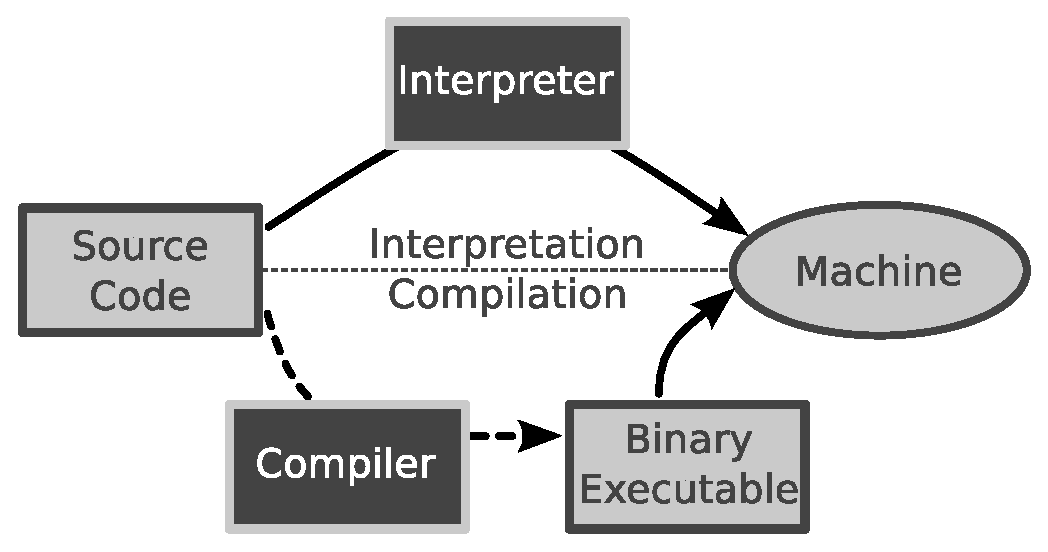
\includegraphics[width=0.6\textwidth]{./graphics/interpreter-vs-compiler.eps}
 \caption{Schematic overview of the difference between translation/compilation and interpretation. Dotted arrows represent translation steps, whereas solid arrows represent execution steps. Interpretation generates has a delay every execution, compilation only requires a (slow) execution step once. This compilation step generates a binary machine-readable file, which can be executed almost directly on the hardware layer of a computer.}
 \label{fig:InterpretationVSCompilation}
\end{figure}

Considering the differences between compilation and interpretation, various cases can be identified where compilation would be preferable over interpretation. In general, compilation is superior when the number of executions desired eliminates the overhead of the compilation procedure (e.g. data fitting). This holds as long as no \MATLAB specific functions or toolboxes are being used, which is mostly not the case for ODE systems.

%TODO: Reference to PUAMAT/CVODE Parser

Furthermore, there is a more specific problem with the build-in \MATLAB solvers, namely that not for every specific situation the most suitable solver is available. For example, large systems of sparsely interlinked differential equations (e.g. Equation \ref{eq:BandedExample}) become time consuming to solve using \MATLAB.
\begin{equation} \label{eq:BandedExample}
  \frac{d\mathbf{F}}{dt} =
  \begin{pmatrix}
   -\alpha_1 & \alpha_2 & 0 & \cdots & \cdots & 0 \\
   \alpha_1 & -\alpha_2 & \alpha_3 & \ddots & \ddots & \vdots \\
   0 & \alpha_2 & -\alpha_3 & \alpha_4  & \ddots & \vdots \\
   \vdots & \ddots & \ddots & \ddots & \ddots & \vdots  \\
   0 & \cdots & \cdots & \cdots & \alpha_{n-1} & -\alpha_{n} \\
  \end{pmatrix}
  \mathbf{F}
\end{equation}
However, suitable solutions for these problems exist. The fast increase of time it takes to solve the system is caused by an exponentially increasing Jacobian matrix. The Jacobian matrix is used by stiff solvers and defined as shown in Equation \ref{eq:Jacobian}.
\begin{equation} \label{eq:Jacobian}
  J_{m,n} =
  \begin{pmatrix}
   \frac{\partial F_1}{\partial x_1} & \cdots & \frac{\partial F_1}{\partial x_n} \\
   \vdots & \ddots & \vdots  \\
   \frac{\partial F_m}{\partial x_1} & \cdots & \frac{\partial F_m}{\partial x_n}
  \end{pmatrix}
\end{equation}
Where $F$ represents the system of ODEs. In the case of an ODE system, $m$ and $n$ are both equal to the number of equations ($N$). This means that the number of elements of the Jacobian matrix increases exponentially, resulting in the following behaviour:
\begin{equation}
 i_{Jac} = N^2 \Rightarrow
 t_{Jac,op} = \Omega(N^2)
\end{equation}
Where $i_{Jac}$ is the number of elements in the Jacobian matrix and $t_{Jac,op}$ the time a typical operation on the Jacobian matrix takes.

In the specific case of Equation \ref{eq:BandedExample}, the Jacobian matrix is a band matrix, which enables specialized matrix handling methods for the Jacobian matrix, which only make $t_{Jac,op}$ increase linearly.

A more general method is the use of a sparse implementation of the Jacobian matrix. This allows elements of the Jacobian matrix not in the center band to be non-zero, in contrast to band matrix implementations. This suite was created to enable \MATLAB to call this type of ODE solvers, following the need to solve large nucleation-elongation ODE systems. These system make use of a cut-off to limit the number of equations, since the exact system consists of an infinite amount of equations. To facilitate the use of a cut-off, the number of equations was left variable and can vary between function calls, without the need to recompile the code.

Next to these specific "sparse Jacobian" solvers, a wide variety of other solvers - all written in the \Fortran programming language - is available through this suite, for an overview see Chapter \ref{ch:Solvers}. The suite consist of the following tools:
\begin{description}
 \item[PPODE\_init] builds the ODE solver libraries and in principle only has to be executed once. See Chapter \ref{ch:Installation}.
 \item[PPODE\_addPaths] loads paths of the \PPODESUITE into the \MATLAB path variable. To access the \PPODESUITE, this function has to be executed. See Chapter \ref{ch:Installation}.
 \item[PPODE\_parser] parses a \MATLAB ODE function to \Fortran. The use of this function eliminates the need for knowledge about the \Fortran programming language. See Chapter \ref{ch:Usage}.
 \item[PPODE\_build] builds the \Fortran function generated by PPODE\_parser. Of course, one can also manually provide a \Fortran function. See Chapter \ref{ch:Usage}.
\end{description}
